\documentclass[12pt, oneside]{article}
\usepackage[letterpaper, margin=1in, headsep=0.5in]{geometry}
\usepackage[english]{babel}
\usepackage[utf8]{inputenc}
\usepackage{amsmath}
\usepackage{amsfonts}
\usepackage{amssymb}
\usepackage{tikz}
\usetikzlibrary{quotes, angles}
\usepackage{graphicx}
%\usepackage{pgfplots}
%\pgfplotsset{width=10cm,compat=1.9}
%\usepgfplotslibrary{statistics}
%\usepackage{pgfplotstable}
%\usepackage{tkz-fct}
%\usepackage{venndiagram}
\usepackage{multicol}


\usepackage{fancyhdr}
\pagestyle{fancy}
\fancyhf{}
\rhead{\thepage \\Name: \hspace{1.5in}.\\}
\lhead{BECA / Dr. Huson / Geometry 10th Grade\\* Unit 4: Parallels and transversals \\ 28 October 2019}

\renewcommand{\headrulewidth}{0pt}

\begin{document}
\subsubsection*{Do Now: Parallelograms \& polygons}

  \begin{enumerate}

\item Given two parallel lines and a transversal, as shown.
\begin{enumerate}
  \item Given $m\angle 7 = 65^\circ$. Find $m\angle 2$. 
  \begin{flushright}
  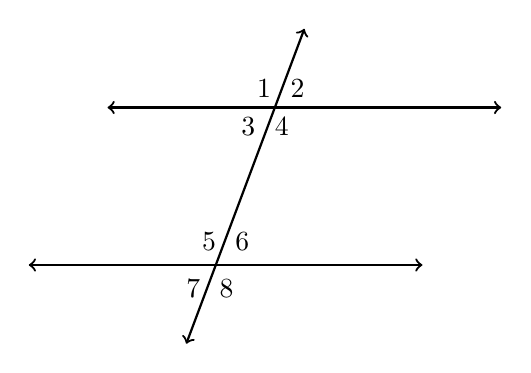
\begin{tikzpicture}
    \draw [<->, thick] (3,2)--(8,2);
    \draw [<->, thick] (2,0)--(7,0);
    \draw [<->, thick] (4,-1)--(5.5,3);
    \node at (4.5,0.3) [left]{$5$};
    \node at (4.5,0.3) [right]{$6$};
    \node at (4.3,-0.3) [left]{$7$};
    \node at (4.3,-0.3) [right]{$8$};
    \node at (5.2,2) [above left]{$1$};
    \node at (5.2,2) [above right]{$2$};
    \node at (5,2) [below left]{$3$};
    \node at (5,2) [below right]{$4$};
  \end{tikzpicture}
  \end{flushright}
    \item State the angle corresponding with $\angle 2$. \vspace{1cm}
    \item Given $m\angle 8 = 115^\circ$ and $m\angle 4 = 5x^\circ$. Find $x$. \vspace{3cm}
    \item What term relates the position of $\angle 4$ to $\angle 5$? \rule{5cm}{0.15mm}
  \end{enumerate}

  \item Given $m\angle R=40$ and $m\angle USR=x+15$, and $m\angle U = x+5$. Find $x$.
  \begin{flushright}
  \begin{tikzpicture}
    %\draw [->, thick] (0,0)--(5,5);
    \draw [<-, thick] (8,0)--(0,0)--(3,3)--(4.5,0);
    \draw [fill] (0,0) circle [radius=0.05] node[below]{$R$};
    \draw [fill] (4.5,0) circle [radius=0.05] node[below]{$S$};
    \draw [fill] (3,3) circle [radius=0.05] node[right]{$U$};
    \draw [fill] (7,0) circle [radius=0.05] node[below]{$T$};
  \end{tikzpicture}
\end{flushright} \vspace{2.5cm}

\item What is the sum of the measures of the internal angles of a pentagon?

\newpage

  \item Given $m\angle M=48$ and $m\angle PNO=110$. Find $m\angle P$.
  \begin{flushright}
    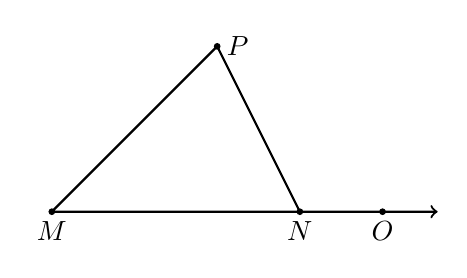
\begin{tikzpicture}[scale=0.7]
      %\draw [->, thick] (0,0)--(5,5);
      \draw [<-, thick] (7,0)--(0,0)--(3,3)--(4.5,0);
      \draw [fill] (0,0) circle [radius=0.05] node[below]{$M$};
      \draw [fill] (4.5,0) circle [radius=0.05] node[below]{$N$};
      \draw [fill] (3,3) circle [radius=0.05] node[right]{$P$};
      \draw [fill] (6,0) circle [radius=0.05] node[below]{$O$};
    \end{tikzpicture}
  \end{flushright}  \vspace{1cm}

\subsubsection*{Circle the appropriate equation and state the justification}
Use the postulates and theorems you have learned. You may abbreviate them as follows: ``def. of bisector," ``$\perp$ rays meet at $90^\circ$," ``complementary $\angle$s add to 90," ``linear pairs add to 180," ``vertical $\angle$s are $\cong$," ``corresponding $\angle$s of $\parallel$ lines are $\cong$."

\item Given $m\angle R=m\angle U =65$, and $m\angle UST=130$. Find $m\angle RSU$.
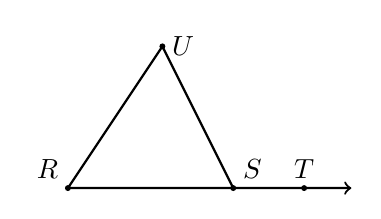
\begin{tikzpicture}[scale=0.6]
  %\draw [->, thick] (0,0)--(5,5);
  \draw [<-, thick] (7,0)--(1,0)--(3,3)--(4.5,0);
  \draw [fill] (1,0) circle [radius=0.05] node[above left]{$R$};
  \draw [fill] (4.5,0) circle [radius=0.05] node[above right]{$S$};
  \draw [fill] (3,3) circle [radius=0.05] node[right]{$U$};
  \draw [fill] (6,0) circle [radius=0.05] node[above]{$T$};
\end{tikzpicture}\\[0.5cm]
$\angle UST \cong \angle RSU$ \hspace{0.5cm} $m\angle UST + m\angle RSU =  180$ \hspace{0.5cm} \rule{6cm}{0.15mm} \vspace{0.25cm}

\item Given $\overrightarrow{BA} \perp \overrightarrow{BC}$, $m \angle ABD = 2x-5$, and $m \angle DBC = x-10$.
  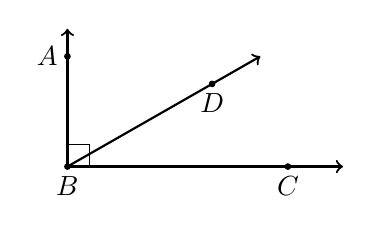
\begin{tikzpicture}[scale=0.7]
    \draw [<->, thick] (0,2.5)--(0,0)--(5,0);
    \draw [->, thick] (0,0)--(3.5, 2);
    \draw [-, thin] (0, 0.4)--(0.4, 0.4)--(0.4, 0);
    \draw [fill] (0,0) circle [radius=0.05] node[below]{$B$};
    \draw [fill] (0,2) circle [radius=0.05] node[left]{$A$};
    \draw [fill] (4,0) circle [radius=0.05] node[below]{$C$};
    \draw [fill] (2.625, 1.5) circle [radius=0.05] node[below]{$D$};
  \end{tikzpicture}\\[0.5cm]
  $\angle ABD \cong \angle DBC$ \hspace{0.5cm} $m\angle ABD + m\angle DBC =  90$ \hspace{0.5cm} \rule{6cm}{0.15mm}


\item $\angle RPS \cong \angle SPU$ \hspace{0.25cm} $m \angle RPS + m \angle SPU = 180^\circ$ \hspace{0.25cm} \rule{6cm}{0.15mm}  \vspace{0.25cm}
    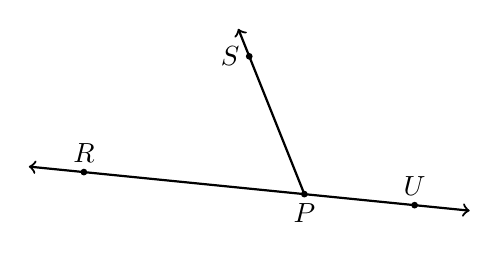
\begin{tikzpicture}[scale=0.7]
      \draw [<->, thick] (-5,.5)--(3,-.3);
      \draw [->, thick] (0,0)--(-1.2,3);
      \draw [fill] (-1,2.5) circle [radius=0.05] node[left ]{$S$};
      \draw [fill] (0,0) circle [radius=0.05] node[below]{$P$};
      \draw [fill] (2,-0.2) circle [radius=0.05] node[above]{$U$};
      \draw [fill] (-4,0.4) circle [radius=0.05] node[above]{$R$};
    \end{tikzpicture}


\item Given $m \angle 1 = 4x+6$, $m \angle 2 = 6x-32$. Find $m \angle 1$.
    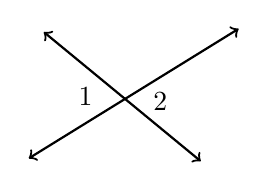
\begin{tikzpicture}[scale=.3, rotate=15]
      \draw [<->, thick] (0,-1.5)--(10,1.5);
      \draw [<->, thick] (2,3.5)--(7,-3.5);
      \node at (3,.4){1};
      \node at (6,-.6){2};
    \end{tikzpicture}\\[0.5cm]
    $\angle 1 \cong \angle 2$ \hspace{1cm} $m\angle 1 + m\angle 2 =  180$ \hspace{0.5cm} \rule{6cm}{0.15mm}

\newpage 
  \item Given $\overrightarrow{BA} \perp \overrightarrow{BC}$, $m \angle ABD = 4x$, and $m \angle DBC = 2x-12$. Find $m \angle DBC$. \\[0.5cm]
  For full credit, show the check using both angle measures.
    \begin{flushleft}
    \begin{tikzpicture}[scale=1.3]
      \draw [<->, thick] (0,3)--(0,0)--(5,0);
      \draw [->, thick] (0,0)--(3.5, 2);
      \draw [-, thin] (0, 0.4)--(0.4, 0.4)--(0.4, 0);
      %\node at (3,.4){1};
      %\node at (6,-.6){2};
      \draw [fill] (0,0) circle [radius=0.05] node[below]{$B$};
      \draw [fill] (0,2) circle [radius=0.05] node[left]{$A$};
      \draw [fill] (4,0) circle [radius=0.05] node[below]{$C$};
      \draw [fill] (2.625, 1.5) circle [radius=0.05] node[below]{$D$};
    \end{tikzpicture}
    \end{flushleft}
    \vspace{3cm}


  \end{enumerate}

\end{document}
